\documentclass[12pt]{report}
\usepackage{fyp_document}
\begin{document}
\chapter{Methodology}
Iris issues and sprints are being tracked using Trello. These are organised using the {\em kanban} system and custom labels inside of Trello. Trello allows filtering of cards by their labels, meaning issues related to a particular sprint can be the only cards visible. This makes tracking sprints and issues for the sprint easy to manage.

\begin{figure}[H]
\begin{tcolorbox}
\begin{center}
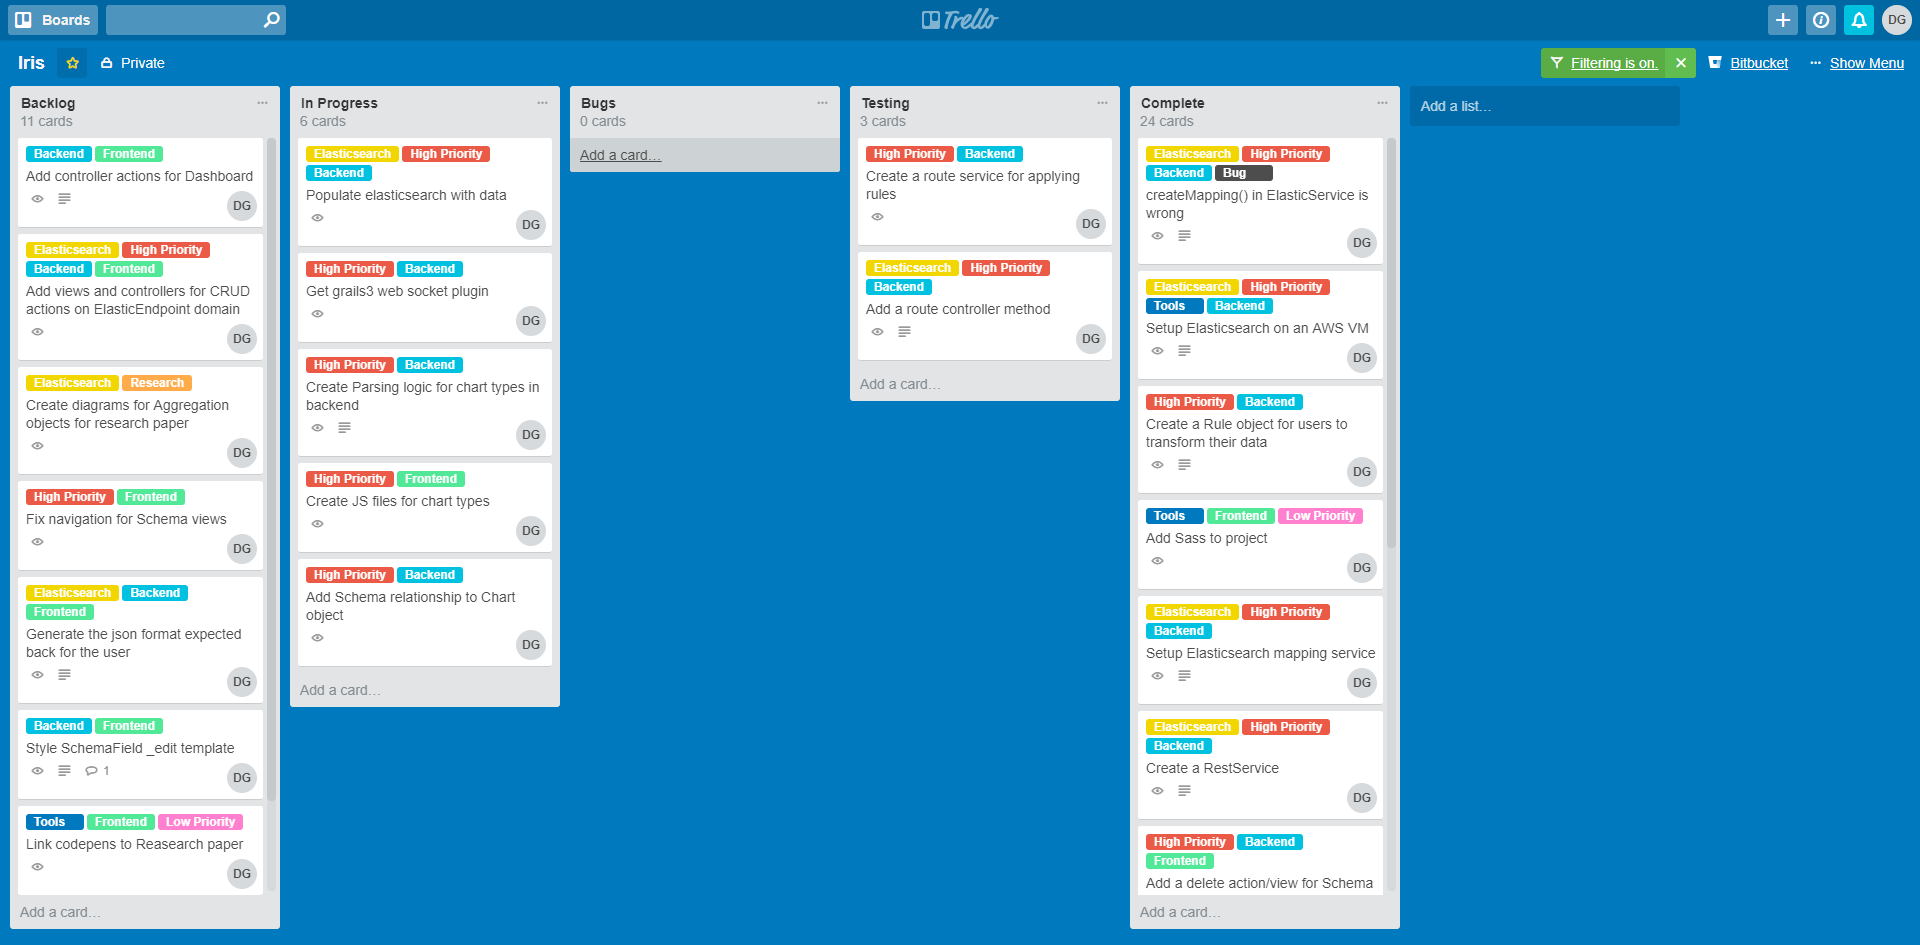
\includegraphics[width=\textwidth,height=\textheight,keepaspectratio]{trello_sprint_2}
\end{center}
\end{tcolorbox}
\caption{Screenshot of the Iris Trello board.}
\end{figure}

\section{Trello}
Trello was used to keep track of issues and sprints in Iris, below are all of the issues for each sprint in Iris. The sprint numbers correspond to the version of Iris at the time of the sprint.
\subsection*{0.0.1}
\begin{itemize}
\item Scope project with Onaware
\item Draw ER Diagram for User owning Dashboards
\item Research d3 wrapper libraries
\item Draw diagrams for Frontend
\item Setup grails 3.3.1 + groovy 2.4.11 + java 8u144 on devices
\item Research Dashboard libraries for serialization
\item Generate Domain classes based off UML diagram
\item Look into Elasticsearch Java api and see if it can be used for building complex aggregations dynamically
\item Use Grails to generate all controllers and views for Domains
\item Add Spring Security Plugin for User Domain
\item Build Elasticsearch Objects
\item Update to latest version of jQuery
\item Update to Bootstrap 4
\item Add controller actions for Schema Domain
\end{itemize}
\subsection*{0.0.2}
\begin{itemize}
\item Style SchemaField edit template
\item Add views and controllers for CRUD actions on ElasticEndpoint domain
\item Generate the json format expected back for the user
\item Fix navigation for Schema views
\item Add levels to javascript aggregation logic
\item Setup Selenide on all machines
\item Create a route service for applying rules
\item Add a route controller method
\item Populate elasticsearch with data
\item Get grails3 web socket plugin
\item Link codepens to Research paper
\item createMapping() in ElasticService is wrong
\item Create diagrams for Aggregation objects for research paper
\item Add Schema relationship to Chart object
\item Setup Elasticsearch on an AWS VM
\item Create a Rule object for users to transform their data
\item Add Sass to project
\item Setup Elasticsearch mapping service
\item Create a RestService
\item Add a delete action/view for Schema domain
\item Deleting Elasticsearch index is not working from front end
\item Create ElasticEndpoint domain
\item Create a Domain for storing Elasticsearch endpoint addresses
\item Research updating Elasticsearch mappings
\item Move over to branch 0.0.2
\item Add Logging to app
\item Add controller actions for Dashboard
\end{itemize}
\subsection*{0.0.3}
\begin{itemize}
\item Display aggregation execution result in playground
\item Schema level counter in JS should match a DOM element to keep it more dynamic
\item Iris demo presentation
\item Write gradle task to kill geckodriver.exe
\item Try adding underscore.js to project to stop javascript error
\item Make aggregations executable in Aggregation Playground
\item Create param link for Schema for routing data
\item Create script to generate data for Iris demo
\item Add Navbar navigation
\item Create Selenide Test for demo
\item Make a test index in Elasticsearch to test out sockets
\end{itemize}
\subsection*{0.0.4}
\begin{itemize}
\item Unsubscribe the chart from onChartLoad
\item Add download chart image button to each chart widget
\item Check if billboard is storing all data points on charts
\item Execute Chart aggregation on dashboard load
\item Add download chart data button to each chart widget
\item Add modal to prompt user for a revision comment when they click update on dashboard
\item Add a dashboard to the bootstrap file
\item Add CRUD functionality to widgets on Dashboard
\item Add update functionality for Dashboards
\item Create XL Modal for dashboards
\item Set and resize chart to be the same as the widget area
\item Create JS files for chart types
\item Dashboard isRendering flag not working in some cases
\item Add date by default to all json objects going into Elasticsearch
\item Create Parsing logic for chart types in backend
\item Load a saved dashboard client side
\item Limit socket messages to dashboards which are currently rendering
\item Save dashboard server side
\item Use browser cache to store a widget's aggregation attribute
\item Use data- HTML attribute for storing widget information
\item billboard.js charts are not displaying correctly
\item Need to add chart Id to subscription charts
\end{itemize}
\subsection*{0.0.5}
\begin{itemize}
\item Add StateChartList to Dashboards
\item Remove all the Grails/Groovy aggregation builder code to reduce code and war size
\item Add titles to charts
\item Add StateChartDisk to Dashboards
\item Add an admin user in production environment for deployment
\item Add revision history for Dashboards
\item Dashboard Revision objects are getting new UID rather than copying older ones
\item Add pattern colours to charts
\item Turn off stompjs debug logging for client speed improvement
\item Change the Aggregation section on Dashboards, to contain a UI rather than raw JSON
\item Edit or Remove extra aggregation attributes from aggregation builder views
\end{itemize}
\subsection*{0.0.6}
\begin{itemize}
\item Accept raw data from data source without running aggregations
\item Add X-Auth-Token header and JWT to each agent
\item Set up VS Code Latex work Shop and config settings in detailed description
\item Add JWT token to prod and dev bootstrap envs
\item Add code editor for creating rules on the schema creation page
\item Add most recent document option to aggregations
\item cloc command
\item Put iris-crypto-rates on raspberry pi and schedule it as a cron job
\item Add dynamic REST call to all agents to grab url  from iris for agent
\item Deploy iris v0.0.6
\end{itemize}
\end{document}